\documentclass[border=5pt]{standalone}
\usepackage{pgfplots}
\pgfplotsset{compat=1.18}
\usepackage{siunitx}
\usepackage{tikz}
\usetikzlibrary{calc}

\definecolor{v2Color}{RGB}{255,127,14}   % Orange for v2
\definecolor{v2resizeColor}{RGB}{44,160,44}   % Green for v2 resize

\begin{document}
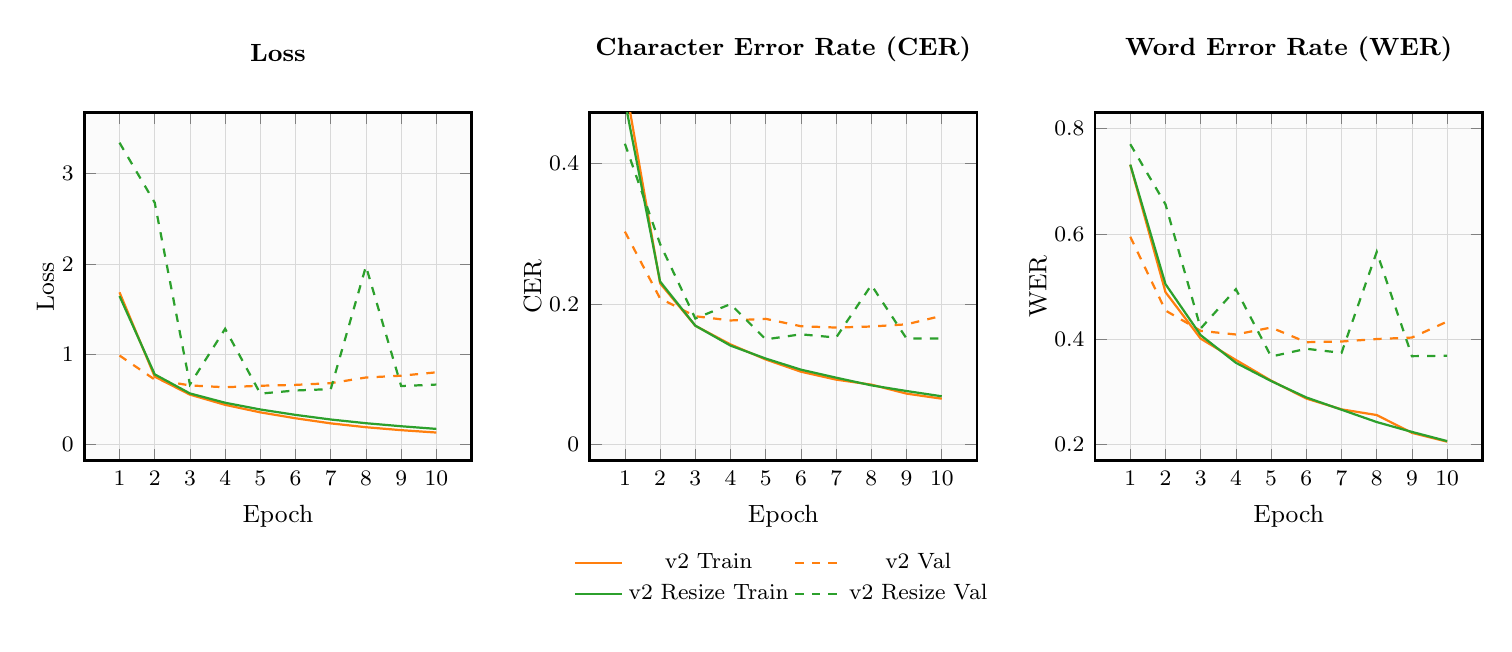
\begin{tikzpicture}[remember picture]

    % Graph 1: Loss
    \begin{axis}[
        name=plot1,
        width=6.5cm,
        height=6cm,
        xlabel={Epoch},
        ylabel={Loss},
        ylabel style={yshift=-0.15cm},
        xmin=0.5, xmax=10.5,
        ymin=0, ymax=3.5,
        xtick={1,2,3,4,5,6,7,8,9,10},
        grid=both,
        grid style={line width=.1pt, draw=gray!10},
        major grid style={line width=.2pt,draw=gray!30},
        title={Loss},
        axis background/.style={fill=gray!3},
        title style={yshift=3mm, font=\small\bfseries},
        label style={font=\small},
        tick label style={font=\footnotesize},
        line width=1pt,
        enlarge x limits=0.05,
        enlarge y limits=0.05,
        every axis plot/.append style={no markers},
        legend to name=commonlegend,
        legend columns=2,
        legend style={draw=none, fill=none, font=\footnotesize}
    ]
        % v2 Train
        \addplot[color=v2Color, thick] coordinates {
            (1, 1.6864) (2, 0.7533) (3, 0.5544) (4, 0.4414) (5, 0.3582)
            (6, 0.2928) (7, 0.2364) (8, 0.1938) (9, 0.1611) (10, 0.1348)
        };
        
        % v2 Validation
        \addplot[color=v2Color, thick, dashed] coordinates {
            (1, 0.9872) (2, 0.7209) (3, 0.6562) (4, 0.6361) (5, 0.6526)
            (6, 0.6623) (7, 0.6813) (8, 0.7440) (9, 0.7637) (10, 0.8013)
        };
        
        % v2 Resize Train
        \addplot[color=v2resizeColor, thick] coordinates {
            (1, 1.6457) (2, 0.7787) (3, 0.5677) (4, 0.4646) (5, 0.3900)
            (6, 0.3302) (7, 0.2791) (8, 0.2381) (9, 0.2046) (10, 0.1752)
        };
        
        % v2 Resize Validation
        \addplot[color=v2resizeColor, thick, dashed] coordinates {
            (1, 3.3421) (2, 2.6788) (3, 0.6672) (4, 1.2830) (5, 0.5658)
            (6, 0.6003) (7, 0.6155) (8, 1.9752) (9, 0.6494) (10, 0.6657)
        };
        
        \legend{v2 Train, v2 Val, v2 Resize Train, v2 Resize Val}
    \end{axis}
    
    % Graph 2: CER, positioned to the right of plot1
    \begin{axis}[
        name=plot2,
        at={($(plot1.east)+(1.5cm,0)$)},
        anchor=west,
        width=6.5cm,
        height=6cm,
        xlabel={Epoch},
        ylabel={CER},
        ylabel style={yshift=-0.15cm},
        xmin=0.5, xmax=10.5,
        ymin=0, ymax=0.45,
        xtick={1,2,3,4,5,6,7,8,9,10},
        grid=both,
        grid style={line width=.1pt, draw=gray!10},
        major grid style={line width=.2pt,draw=gray!30},
        title={Character Error Rate (CER)},
        axis background/.style={fill=gray!3},
        title style={yshift=3mm, font=\small\bfseries},
        label style={font=\small},
        tick label style={font=\footnotesize},
        line width=1pt,
        enlarge x limits=0.05,
        enlarge y limits=0.05,
        every axis plot/.append style={no markers}
    ]
        % v2 Train
        \addplot[color=v2Color, thick] coordinates {
            (1, 0.5158) (2, 0.2296) (3, 0.1693) (4, 0.1427) (5, 0.1213)
            (6, 0.1039) (7, 0.0926) (8, 0.0855) (9, 0.0727) (10, 0.0655)
        };
        
        % v2 Validation
        \addplot[color=v2Color, thick, dashed] coordinates {
            (1, 0.3032) (2, 0.2081) (3, 0.1828) (4, 0.1768) (5, 0.1791)
            (6, 0.1686) (7, 0.1667) (8, 0.1682) (9, 0.1713) (10, 0.1834)
        };
        
        % v2 Resize Train
        \addplot[color=v2resizeColor, thick] coordinates {
            (1, 0.4890) (2, 0.2322) (3, 0.1694) (4, 0.1410) (5, 0.1226)
            (6, 0.1068) (7, 0.0954) (8, 0.0845) (9, 0.0764) (10, 0.0689)
        };
        
        % v2 Resize Validation
        \addplot[color=v2resizeColor, thick, dashed] coordinates {
            (1, 0.4282) (2, 0.2856) (3, 0.1796) (4, 0.2001) (5, 0.1499)
            (6, 0.1571) (7, 0.1525) (8, 0.2272) (9, 0.1510) (10, 0.1510)
        };
    \end{axis}
    
    % Graph 3: WER, positioned to the right of plot2
    \begin{axis}[
        name=plot3,
        at={($(plot2.east)+(1.5cm,0)$)},
        anchor=west,
        width=6.5cm,
        height=6cm,
        xlabel={Epoch},
        ylabel={WER},
        ylabel style={yshift=-0.15cm},
        xmin=0.5, xmax=10.5,
        ymin=0.2, ymax=0.8,
        xtick={1,2,3,4,5,6,7,8,9,10},
        grid=both,
        grid style={line width=.1pt, draw=gray!10},
        major grid style={line width=.2pt,draw=gray!30},
        title={Word Error Rate (WER)},
        axis background/.style={fill=gray!3},
        title style={yshift=3mm, font=\small\bfseries},
        label style={font=\small},
        tick label style={font=\footnotesize},
        line width=1pt,
        enlarge x limits=0.05,
        enlarge y limits=0.05,
        every axis plot/.append style={no markers}
    ]
        % v2 Train
        \addplot[color=v2Color, thick] coordinates {
            (1, 0.7310) (2, 0.4895) (3, 0.4012) (4, 0.3608) (5, 0.3216)
            (6, 0.2876) (7, 0.2671) (8, 0.2563) (9, 0.2225) (10, 0.2058)
        };
        
        % v2 Validation
        \addplot[color=v2Color, thick, dashed] coordinates {
            (1, 0.5945) (2, 0.4546) (3, 0.4160) (4, 0.4091) (5, 0.4223)
            (6, 0.3945) (7, 0.3958) (8, 0.4005) (9, 0.4033) (10, 0.4336)
        };
        
        % v2 Resize Train
        \addplot[color=v2resizeColor, thick] coordinates {
            (1, 0.7314) (2, 0.5046) (3, 0.4078) (4, 0.3554) (5, 0.3208)
            (6, 0.2897) (7, 0.2664) (8, 0.2430) (9, 0.2243) (10, 0.2069)
        };
        
        % v2 Resize Validation
        \addplot[color=v2resizeColor, thick, dashed] coordinates {
            (1, 0.7701) (2, 0.6560) (3, 0.4206) (4, 0.4950) (5, 0.3673)
            (6, 0.3820) (7, 0.3743) (8, 0.5658) (9, 0.3680) (10, 0.3688)
        };
    \end{axis}

    % Positioning the common legend below all graphs
    \node at ($(plot1.south)!0.5!(plot3.south)+(0,-1.5cm)$) {\pgfplotslegendfromname{commonlegend}};
    
\end{tikzpicture}
\end{document}